\chapter{Structure} \label{chap_structure}

A thesis must be a coherent document of a research project, not a collection of loosely connected pages. This chapter walks through the typical structure of a thesis from cover to cover, and discusses the aim and content of each part. Sections \ref{sec_coverpage} through \ref{sec_declaration} describe the mandatory pages that must be included in each thesis.

\section{Cover page} \label{sec_coverpage}

The cover page is officially provided by THL and signed by the supervisor and the board of examinations, as can be seen at the first page of this document and in Figure \ref{fig:coverpage}. Students will receive an original version and a black-white copy of the official cover page, each of which serves as the cover of the two thesis copies.

\begin{figure}[htb]
  \centering
  
\includegraphics[scale=.8]{titlepage_small}\\
  \caption{Example of a page 1 - Cover page}\label{fig:coverpage}
\end{figure}

\section{Task description}

The task description covers some background information about the thesis, lists the major steps during the work, and specifies the deliverables of the thesis. It can be seen as a contract between the student and the supervisor or the company and is the basis for grading. Therefore, students should make sure the listed tasks are reasonable to be finished within the time constraints. Figure \ref{fig:task} shows an example of this page.

\begin{figure}[htb]
  \centering
  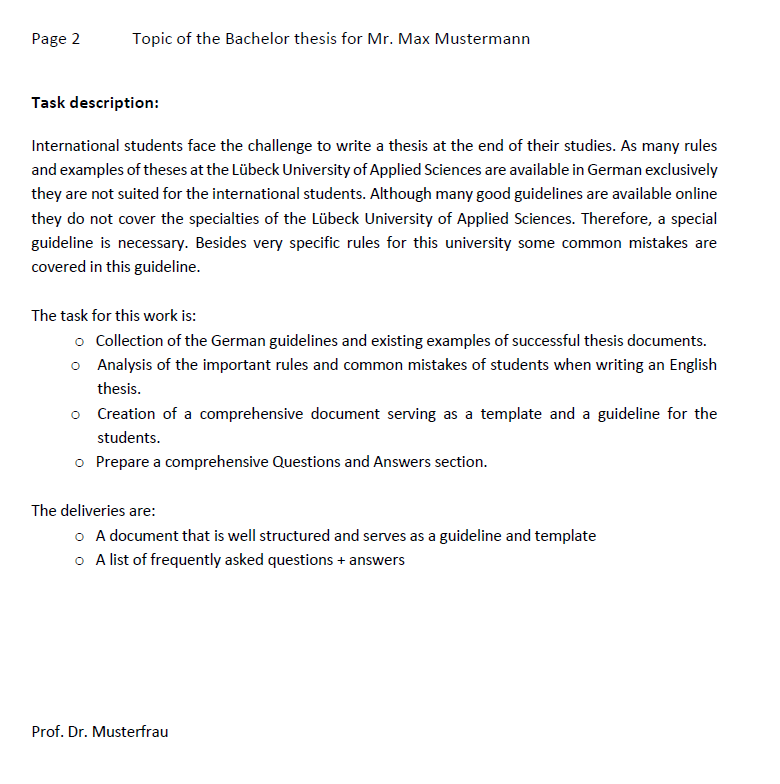
\includegraphics[scale=.8]{thesistask_small}\\ 
  \caption{Example of a page 2 - Task description}\label{fig:task}
\end{figure}

\section{Declaration} \label{sec_declaration}

Students are required to sign the declaration of the thesis provided by THL (see Figure \ref{fig:declaration}), which includes \cite{kun08}:
\begin{itemize}
\item The fact that she or he writes the work independently without outside help.
\item The fact that she or he has used only the cited sources.
\item The fact that she or he agrees with a publication of the work.
\end{itemize}

The first two items are mandatory while the last one is optional. Pay attention that some students working in companies are required to sign a Non-Disclosure Agreement (NDA) with the companies, and some companies do not agree to publish the thesis work. In this case, the last paragraph must be removed from the declaration.

%Figure from pdf file - preferred option since it allows to include true vector graphics 
\begin{figure}[htb]
  \centering
  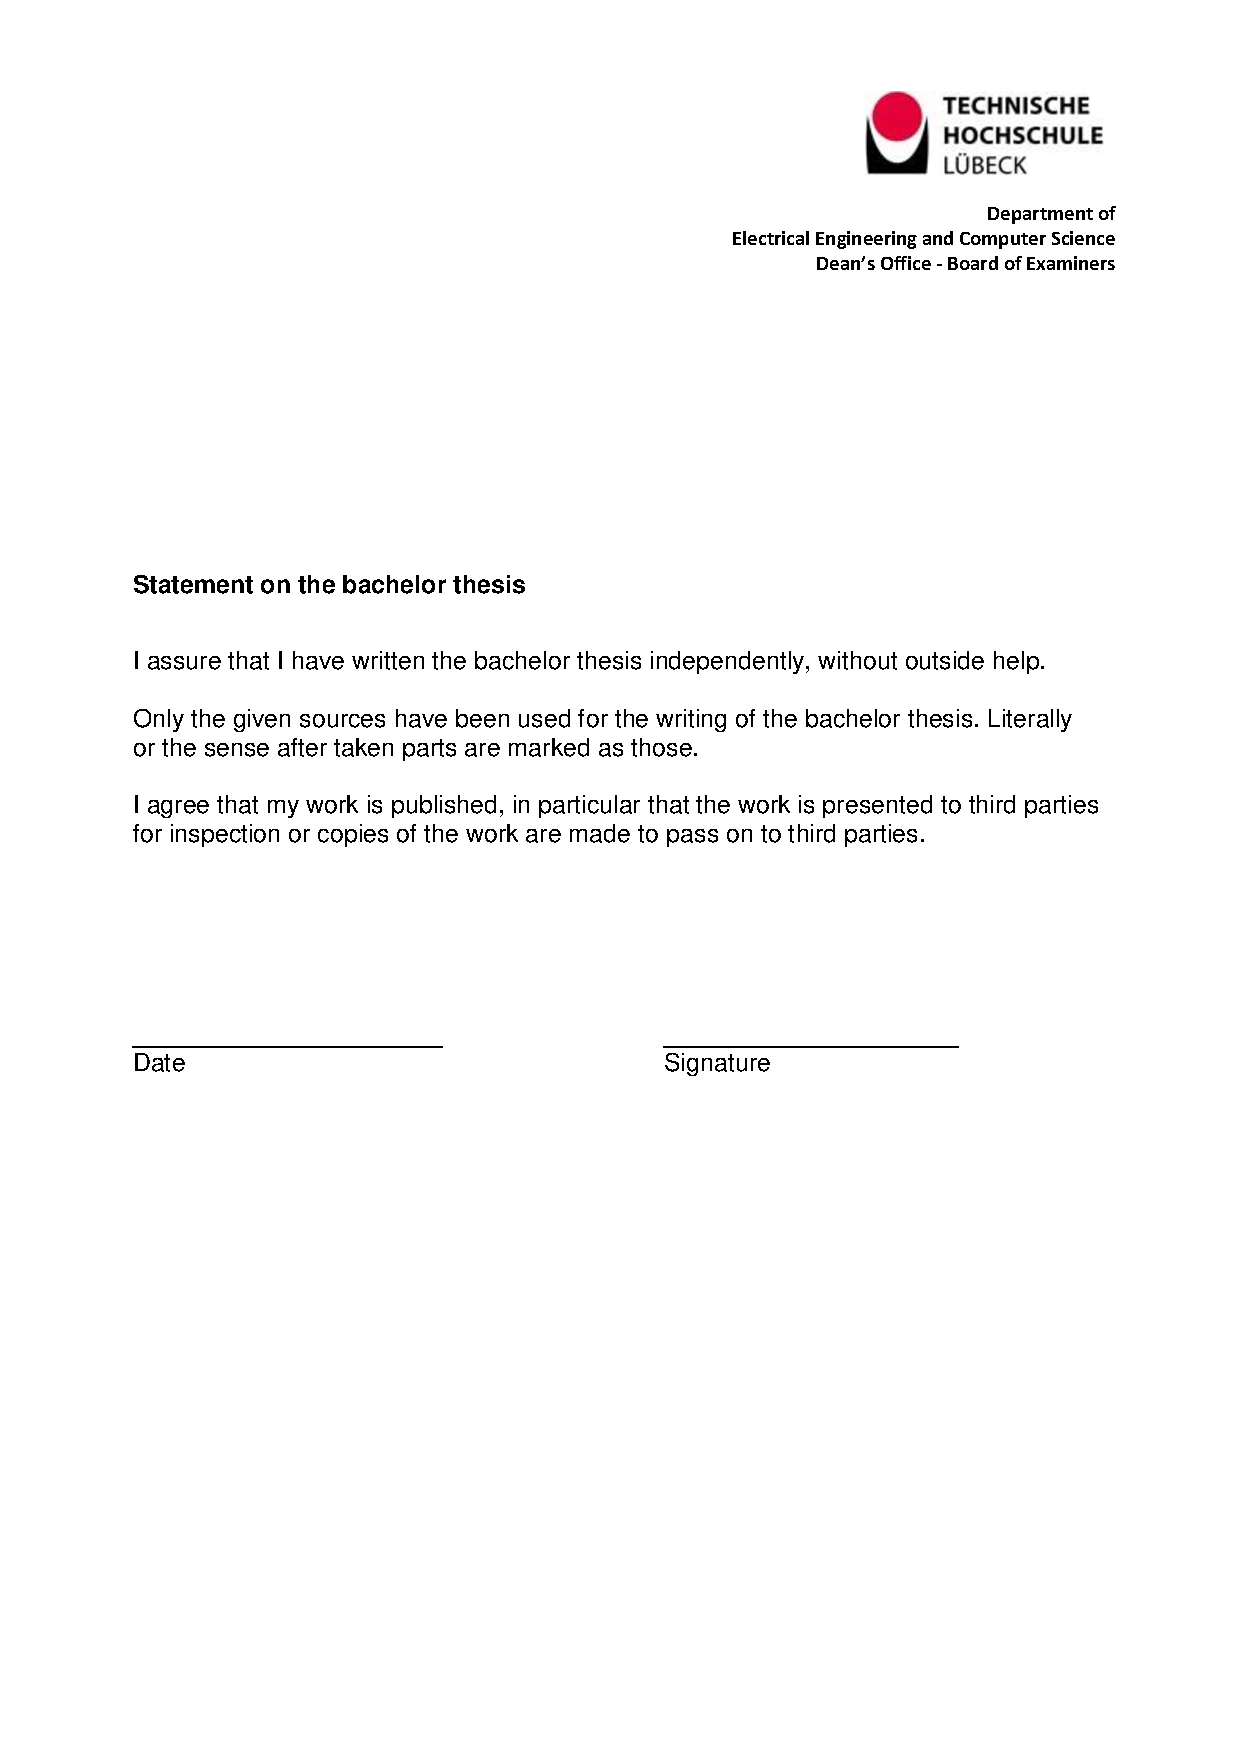
\includegraphics[scale=.4]{thesis_statement}\\ % PDF-File
  \caption{Declaration form}\label{fig:declaration}
\end{figure}

\section{Abstract}

The abstract is one page maximum, including information from the cover sheet plus the abstract of the work. By default the secretariat will hand out a form that the students can fill in. Many students, however, have developed their own page for this purpose. 

The abstract is one of the most important parts of a thesis, because it leaves the very \textit{first impression} of the following text. It has to be \textit{self-contained}, which means it can be understood separately from the thesis itself. 

\section{Table of contents}

A table of contents is a list of all chapters and sections with page numbers. It enables the readers to easily find information they are looking for. A LaTeX command automatically generates the table of contents.

The titles of chapters and sections should have a good naming so that the reader can easily imagine what the content is about. This is important if the thesis is briefly read by someone (e.g.~from a company that considers to hire the student) in the future who wants to get an impression whether the work has been carried out in a good way.

The work should be provided as a pdf file later. It is nice if the table on contents is linked with the sections so that a click on a section title in the table of contents leads to a jump into the section. A similar functionality should also be provided for other links (e.g.~to the bibliography). This functionality is already contained in this LaTeX template, but should be conserved when converting it into pdf.

\section{Chapter 1: Introduction}

The purpose of the introduction is to stimulate the readers' interest and guide the reader into the subject. Before writing a good introduction usually the author needs to know the body of the thesis, so it is suggested to write the introduction after completing the rest of the thesis.

An introduction typically contains 3 basic parts \cite{les06}:
\begin{itemize}
\item Background or motivation of the thesis
\item Goal of the thesis
\item Organization of the following chapters 
\end{itemize}

The first part briefly states what the problem is and why it is desired to address this problem in the thesis. The second part presents the goal to be achieved in this thesis, i.e. solution to this problem. It is not a good idea to transfer the text from the task description into this chapter. Students are expected to explain the problem and the goal in their own words. Finally,  a preview of the rest of the document should be provided chapter by chapter to tell the reader what can be expected.

The benefit of a preview is that the reader will be able to scan the thesis at first and have a good sense of what will be covered in each chapter. This allows the reader to select individual chapters if she or he wants to skip parts of the document. To make the thesis as readable as possible, it is suggested to use this strategy throughout the thesis by writing an introductory paragraph at the beginning of each chapter (or even some sections if necessary). See the beginning of the next section for a simple example.
  
\section{Chapter 2 to N-1: Main body} 

The body is the major component of the thesis. It describes how the author accomplished the task step by step and how she or he achieved the results. There is no fixed structure of the main body, as it may vary according to the task description, but Section \ref{sec_examplestructure} describes a common way of organizing the chapters. Section \ref{sec_pitfall} introduces a common pitfall in writing the main body the thesis.

\subsection{Example organization} \label{sec_examplestructure}

In computer science topics there is often a task description which foresees the development of a theoretical concept combined with a prototypical implementation. The following outline can be used in this case.

In the second chapter the problem is analyzed in depth by using one or several scenarios. At the end of the chapter there is a list of requirements which have to be fulfilled to provide a solution to the problem. The requirements do not have to be pure technical requirements, but may include license issues and economic constraints (e.g.~low investment costs).

In the third chapter literature and related work (in standardization documents, research papers, and existing systems) is examined whether there is already a solution to the problem. This should not be the case because the work would otherwise already be finished in this chapter. At the end of this chapter a table is provided which shows the examination results and details which requirements are fulfilled by each existing approach. All related work has to cover some smaller or bigger part of the requirements. Otherwise, they cannot be regarded as related work, but it is necessary to point out their deficits with respect to the problem.

In chapter four a theoretical approach to the problem is drafted. Often a basic idea for the solution of the problem is presented at the beginning which is elaborated afterwards. At the end of the chapter the developed solution is compared to the requirements to verify whether all of them are fulfilled. This should be the case for the mandatory requirements. Some optional requirements may not or partially be fulfilled.

In the fifth chapter a practical implementation of the theoretical concept is presented. Technical information on the implementation is given, e.g.~used programming languages, development tools, hardware, etc. This chapter demonstrates that the theoretical solution works in reality.

It is important to note that the structure of the thesis does not match to the actual way how the thesis subject has been addressed. For many chapters material is collected at the beginning and is drafted as bullet point lists. Towards the end of the thesis time it is converted into text. In addition, it has to be checked before the start of the thesis that there is no perfect solution available for the problem which can be applied easily.

The first advisor for the thesis can give recommendations on how to structure the thesis. A discussion on this should happen relatively early after the start of the thesis.

\subsection{A common pitfall} \label{sec_pitfall}

While writing a thesis, the student has only limited time, energy and number of pages to describe the work which has been accomplished. Hence, some parts need to be elaborated while others just briefly mentioned. In general, it depends on the significance of the particular part of the work. 

However, one common pitfall is that some students devote too many pages describing the detailed software implementation and put many blocks of code in their thesis. Even if the majority of the thesis is about software implementation, one should not describe too many details of the source code. What should be elaborated and emphasized is the class interfaces, program framework, design considerations and implementation trade-offs behind the trivial details. As will be mentioned in Section \ref{sec_CD}, an enclosed CD will provide the entire source code for reference. Consequently, include source code only when it helps to clarify significant issues.

\section{Chapter n: Conclusion and outlook}

The final chapter comprises the major results of the thesis and the outlook. It summarizes the achievement and the results of the work in technical terms. At this point it can be assumed that the previous chapters of the thesis are known to the reader (in contrast to the summary at the beginning). Nevertheless, it should be taken into account that there are quick readers who have skipped several chapters and just want to have an impression of the major findings of the work.

The outlook proposes future possible extensions or challenges of this work. Optional requirements which have not or only partially been fulfilled may give a hint for this.


\section{Acknowledgements}

The author is free to acknowledge the supervisor(s) and anyone who helped the author: 
\begin{itemize}
\item Technically (including materials, supplies)
\item Intellectually (assistance, advice)
\item Financially (for example, departmental support, travel grants, parents)
\end{itemize}

\section{Appendices}

Appendices can include the list of figures, tables or listings and other materials which are either too long to be inserted into the main chapters of the thesis, or which are interesting, but not essential to understand the main text \cite{les06}.

\section{Bibliography or references}

In this section, the student should provide a list of referenced literature in alphabetical order or in the order that the references appear in the main text. Each entry in the bibliography has to be mentioned at least once in the main text. For the formatting of bibliography, please refer to Section \ref{sec_citations}.

\section{Enclosed CD} \label{sec_CD}

If software implementation is an important part of the thesis, it is recommended that a CD containing the source code be enclosed on the back cover of the thesis.

\endinput 